% =====================================================================
%  hc_grid_v1.tex  --  Hydrocode sheet, Fig. 1: the staggered grid
%  CARTOON (line art only, no numbers): three cells k-1, k, k+1 of one
%  material.  Faces carry half-integer indices and the velocity u;
%  centers carry integer indices and rho, e, P, q, c.  Brackets show the
%  cell mass M_k (face to face) and the node mass (M_k + M_{k+1})/2
%  (center to center) that the momentum update divides by.
%  Unequal widths are deliberate: cells deform, mass per cell does not.
% =====================================================================
\documentclass[tikz,border=6pt]{standalone}
\usepackage{amsmath,bm}
\usetikzlibrary{arrows.meta,decorations.pathreplacing}
\definecolor{slate}{HTML}{2C3E50}
\definecolor{oiblue}{HTML}{0072B2}
\definecolor{oiorange}{HTML}{E69F00}
\definecolor{oivermil}{HTML}{D55E00}
\begin{document}
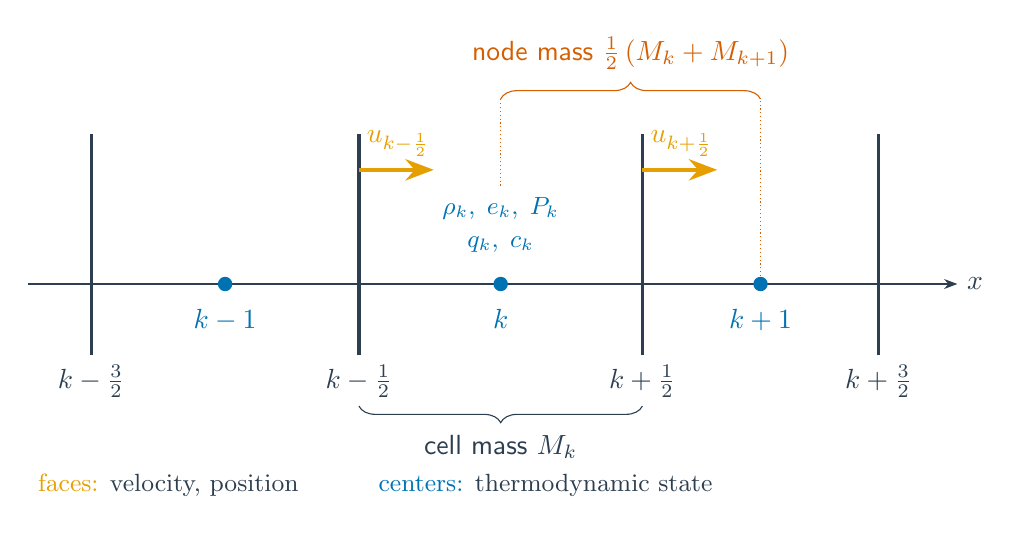
\begin{tikzpicture}[font=\sffamily, text=slate, >=Stealth]
  % faces at x = 0, 3.4, 7.0, 10.0  (cells of unequal width)
  \def\fa{0}\def\fb{3.4}\def\fc{7.0}\def\fd{10.0}
  \draw[->,slate,thin] (-0.8,0) -- (11.0,0) node[right] {$x$};
  \foreach \f in {\fa,\fb,\fc,\fd} \draw[slate,line width=1.2pt] (\f,-0.9) -- (\f,1.9);
  \foreach \c/\lab in {1.7/{k-1}, 5.2/{k}, 8.5/{k+1}} {
    \fill[oiblue] (\c,0) circle (2.6pt);
    \node[below=4pt, text=oiblue] at (\c,-0.05) {$\lab$};
  }
  \node[below] at (\fa,-0.9) {$k-\tfrac{3}{2}$};
  \node[below] at (\fb,-0.9) {$k-\tfrac{1}{2}$};
  \node[below] at (\fc,-0.9) {$k+\tfrac{1}{2}$};
  \node[below] at (\fd,-0.9) {$k+\tfrac{3}{2}$};
  % velocities on faces
  \foreach \f/\lab in {\fb/{u_{k-\frac{1}{2}}}, \fc/{u_{k+\frac{1}{2}}}} {
    \draw[->,oiorange,line width=1.6pt] (\f,1.45) -- ++(0.95,0);
    \node[above,text=oiorange] at (\f+0.5,1.5) {$\lab$};
  }
  % thermodynamic state at center k
  \node[text=oiblue, align=center, font=\small] at (5.2,0.75) {$\rho_k,\;e_k,\;P_k$\\[1pt] $q_k,\;c_k$};
  % cell mass bracket (face to face)
  \draw[decorate,decoration={brace,amplitude=6pt,mirror},slate] (\fb,-1.55) -- (\fc,-1.55)
      node[midway,below=7pt] {cell mass $M_k$};
  % node mass bracket (center to center)
  \draw[decorate,decoration={brace,amplitude=6pt},oivermil] (5.2,2.35) -- (8.5,2.35)
      node[midway,above=7pt,text=oivermil] {node mass $\tfrac{1}{2}\left(M_k+M_{k+1}\right)$};
  \draw[densely dotted,oivermil] (5.2,1.25) -- (5.2,2.35);
  \draw[densely dotted,oivermil] (8.5,0.1) -- (8.5,2.35);
  \node[anchor=west,font=\small] at (-0.8,-2.55) {\textcolor{oiorange}{faces:} velocity, position \hspace{8mm} \textcolor{oiblue}{centers:} thermodynamic state};
\end{tikzpicture}
\end{document}
